%%%%%%%%%%%%%%%%%%%%%%%%%%%%%%%%%%%%%%%%%%%%%%%%%%%%%%%%%%%%%%%%%%%%%%%%%%%%
% AGUtmpl.tex: this template file is for articles formatted with LaTeX2e,
% Modified November 2013
%
% This template includes commands and instructions
% given in the order necessary to produce a final output that will
% satisfy AGU requirements.
%
% PLEASE DO NOT USE YOUR OWN MACROS
% DO NOT USE \newcommand, \renewcommand, or \def.
%
% FOR FIGURES, DO NOT USE \psfrag
%
%%%%%%%%%%%%%%%%%%%%%%%%%%%%%%%%%%%%%%%%%%%%%%%%%%%%%%%%%%%%%%%%%%%%%%%%%%%%
%
% All questions should be e-mailed to latex@agu.org.
%
%%%%%%%%%%%%%%%%%%%%%%%%%%%%%%%%%%%%%%%%%%%%%%%%%%%%%%%%%%%%%%%%%%%%%%%%%%%%
%
% Step 1: Set the \documentclass
%
% There are two options for article format: two column (default)
% and draft.
%
% PLEASE USE THE DRAFT OPTION TO SUBMIT YOUR PAPERS.
% The draft option produces double spaced output.
%
% Choose the journal abbreviation for the journal you are
% submitting to:

% jgrga JOURNAL OF GEOPHYSICAL RESEARCH
% gbc   GLOBAL BIOCHEMICAL CYCLES
% grl   GEOPHYSICAL RESEARCH LETTERS
% pal   PALEOCEANOGRAPHY
% ras   RADIO SCIENCE
% rog   REVIEWS OF GEOPHYSICS
% tec   TECTONICS
% wrr   WATER RESOURCES RESEARCH
% gc    GEOCHEMISTRY, GEOPHYSICS, GEOSYSTEMS
% sw    SPACE WEATHER
% ms    JAMES
% ef    EARTH'S FUTURE
%
%
%
% (If you are submitting to a journal other than jgrga,
% substitute the initials of the journal for "jgrga" below.)

\documentclass[draft, grl]{agutexSI}
\usepackage{graphicx}


%%%%%%%%%%%%%%%%%%%%%%%%%%%%%%%%%%%%%%%%%%%%%%%%%%%%%%%%%%%%%%%%%%%%%%%%%
%
%  SUPPORTING INFORMATION TEMPLATE
%
%% ------------------------------------------------------------------------ %%
%
%
%Please use this template when formatting and submitting your Supporting Information.

%This template serves as both a “table of contents” for the supporting information for your article and as a summary of files.
%
%
%OVERVIEW
%
%Please note that all supporting information will be peer reviewed with your manuscript.
%In general, the purpose of the supporting information is to enable authors to provide and archive auxiliary information such as data %tables, method information, figures, video, or computer software, in digital formats so that other scientists can use it.
%The key criteria are that the data:
% 1. supplement the main scientific conclusions of the paper but are not essential to the conclusions (with the exception of
%    including %data so the experiment can be reproducible);
% 2. are likely to be usable or used by other scientists working in the field;
% 3. are described with sufficient precision that other scientists can understand them, and
% 4. are not exe files.
%
%USING THIS TEMPLATE
%
%***All references should be included in the reference list of the main paper so that they can be indexed, linked, and counted as citations.  The reference section does not count toward length limits.
%
%All Supporting text and figures should be included in this document. Insert supporting information content into each appropriate section of the template. %Figures and tables should appear above each caption.  To add additional captions, simply copy and paste each sample caption as needed.

%Tables may be included, but can also be uploaded separately, especially if they are larger than 1 page, or if necessary for retaining table formatting. Data sets, large tables, movie files, and audio files should be uploaded separately, following AGU naming conventions. Include their captions in this document and list the file name with the caption. You will be prompted to upload these files on the Upload Files tab during the submission process, using file type “Supporting Information (SI)”

%IMPORTANT NOTE ON FIGURES AND TABLES
% Placeholders for figures and tables appear after the \end{article} command, after references.
% DO NOT USE \psfrag or \subfigure commands.
%
%  Uncomment the following command to include .eps files
 % \usepackage[dvips]{graphicx}
%
%  Uncomment the following command to allow illustrations to print
%   when using Draft:
%  \setkeys{Gin}{draft=false}
%
% Substitute one of the following for [dvips] above
% if you are using a different driver program and want to
% proof your illustrations on your machine:
%
% [xdvi], [dvipdf], [dvipsone], [dviwindo], [emtex], [dviwin],
% [pctexps],  [pctexwin],  [pctexhp],  [pctex32], [truetex], [tcidvi],
% [oztex], [textures]
%
%
%% ------------------------------------------------------------------------ %%
%
%  ENTER PREAMBLE
%
%% ------------------------------------------------------------------------ %%

% Author names in capital letters:
%\authorrunninghead{BALES ET AL.}

% Shorter version of title entered in capital letters:
%\titlerunninghead{SHORT TITLE}

%Corresponding author mailing address and e-mail address:
%\authoraddr{Corresponding author: A. B. Smith,
%Department of Hydrology and Water Resources, University of
%Arizona, Harshbarger Building 11, Tucson, AZ 85721, USA.
%(a.b.smith@hwr.arizona.edu)}

\begin{document}

%% ------------------------------------------------------------------------ %%
%
%  TITLE
%
%% ------------------------------------------------------------------------ %%

%\includegraphics{agu_pubart-white_reduced.eps}


\title{Supporting Information for ``Microburst Scale Size Derived from Multiple Bounces of a Microburst Simultaneously Observed with the FIREBIRD-II CubeSats"}
%
% e.g., \title{Supporting Information for "Terrestrial ring current:
% Origin, formation, and decay $\alpha\beta\Gamma\Delta$"}
%
%DOI: 10.1002/%insert paper number here%

%% ------------------------------------------------------------------------ %%
%
%  AUTHORS AND AFFILIATIONS
%
%% ------------------------------------------------------------------------ %%

\authors{Mykhaylo Shumko\altaffilmark{1}, John Sample\altaffilmark{1}, Arlo Johnson\altaffilmark{1}, Bern Blake\altaffilmark{2}, Alex Crew\altaffilmark{3}, Harlan Spence\altaffilmark{4}, David Klumpar\altaffilmark{1}, Oleksiy Agapitov\altaffilmark{5}, Matthew Handley\altaffilmark{1}}

\altaffiltext{1}{Department of Physics, Montana State University, Bozeman, Montana, USA}
\altaffiltext{2}{Space Science Applications Laboratory, The Aerospace Corporation, Los Angeles, California, USA}
\altaffiltext{3}{The Johns Hopkins University Applied Physics Laboratory LLC, Laurel, Maryland, USA}
\altaffiltext{4}{Institute for the Study of Earth, Oceans, and Space, University of New Hampshire, Durham, New Hampshire, USA}
\altaffiltext{5}{Space Sciences Laboratory, UC Berkeley, Berkeley, California, USA}

\lefthead{Shumko et al.}
\righthead{Microburst Scale Size Derived From a Bouncing Microburst}

%Use \author{\altaffilmark{}} and \altaffiltext{}

% \altaffilmark will produce footnote;
% matching \altaffiltext will appear at bottom of page.

% \authors{A. B. Smith,\altaffilmark{1}
% Eric Brown,\altaffilmark{1,2} Rick Williams,\altaffilmark{3}
% John B. McDougall\altaffilmark{4}, and S. Visconti\altaffilmark{5}}

%\altaffiltext{1}{Department of Hydrology and Water Resources,
%University of Arizona, Tucson, Arizona, USA.}

%\altaffiltext{2}{Department of Geography, Ohio State University,
%Columbus, Ohio, USA.}

%\altaffiltext{3}{Department of Space Sciences, University of
%Michigan, Ann Arbor, Michigan, USA.}

%\altaffiltext{4}{Division of Hydrologic Sciences, Desert Research
%Institute, Reno, Nevada, USA.}

%\altaffiltext{5}{Dipartimento di Idraulica, Trasporti ed
%Infrastrutture Civili, Politecnico di Torino, Turin, Italy.}



%% ------------------------------------------------------------------------ %%
%
%  BEGIN ARTICLE
%
%% ------------------------------------------------------------------------ %%

% The body of the article must start with a \begin{article} command
%
% \end{article} must follow the references section, before the figures
%  and tables.

\begin{article}

%% ------------------------------------------------------------------------ %%
%
%  TEXT
%
%% ------------------------------------------------------------------------ %%



\noindent\textbf{Contents of this file}
%%%Remove or add items as needed%%%
\begin{enumerate}
%\item Introduction to supporting information
\item Time and position correction
\item Figures S1-S6
\end{enumerate}

\iffalse
\noindent\textbf{Introduction}
%Type or paste your text here. The introduction gives a brief overview of the supporting information. You should include information %about as many of the following as possible (when appropriate):
% 1. a general overview of the kind of data files;
% 2. information about when and how the data were collected or created;
% 3. a general description of processing steps used;
% 4. any known imperfections or anomalies in the data.

The following supporting material describes the method we used to calculate the time difference and separation between FU3 and FU4 at 06:12 UT on February 2nd, 2015.

We used two types of events that FIREBIRD-II observed on February 2nd, 2015 with a unique time lag signature. The first event type is a microburst or trains of microbursts that were assumed to hit both spacecraft simultaneously, even if the data was not time stamped at the same time due to their clock difference. The other type of event used to calculate the FU3-FU4 separation were stationary structures (sudden increase or decrease of electron count rate).
\fi


\noindent\textbf{Time and position correction} 

We used the following method to calculate the clock difference, $\delta t_{c}$  and separation, $d$ between FU3 and FU4 at 06:12 UT on February 2nd, 2015.

The relative clock difference was calculated with a cross-correlation time lag analysis on uniquely-identified trains of microbursts that hit both spacecraft simultaneously. Four time periods with coincident microbursts were hand-picked on February 2nd, 2015 and are shown in Figs. \ref{figure_S1}-\ref{figure_S4}, panels (a) and (b). The cross-correlation time lag analysis was applied to the HiRes time series in panels (a) and (b), and the resulting normalized cross-correlation coefficient as a function of time is shown in panel (c). To validate the peak lag identified in panel (c), FU3's time series was shifted by that lag and is shown in panel (d).

The clock differences from the simultaneous microbursts in Figs. \ref{figure_S1}-\ref{figure_S4} were linearly fit to account for the relative clock drift (${\approx} 20$ ms/hour at this time), giving a value of $\delta t_{c} = 2.28 \pm 0.12 \ s$ at the time of the microburst analyzed here. This time shift was applied to the HiRes data in Fig. 1. A clock difference of $\delta t_{c}  = 2.45^{+ 0.51}_{-0.98}$ s was independently calculated with the FIREBIRD-II telemetry beacon time stamps that were downlinked during operational passes.

We calculate the spacecraft separation, by applying same the cross-correlation time lag analysis on structures assumed to be spatial and are shown in Figs. \ref{figure_S5} and \ref{figure_S6}. The lag from the peak cross-correlation between these events is a sum of the clock difference and time lag due to the spacecraft separation. We interpret the time lag due to the spacecraft separation as the time difference between when the leading satellite observed a stationary spatial feature, to when the trailing satellite observed the same stationary spatial feature. With the method described above, we find the spatial time lag to be $\delta t_{d} = 2.64 \pm 0.12$ s (after we account for the clock difference and its uncertainty). To convert from a spatial time lag to a spacecraft separation, we calculate the satellite velocity. We calculate the velocity using a Two Line Element (TLE), a data format containing the orbit parameters that are used for orbit propagation. With the TLE derived spacecraft velocity, $v = 7.57 \ km/s$, the spacecraft separation was $d = 19.9 \pm 0.9 \ km $.

An independent method to calculate the spacecraft separation was developed. The separation was calculated using TLEs. The TLE from February 2nd was anomalous and was not used in this analysis. Instead, seven TLEs released up to five days after the microburst event were backpropagated, using the SGP-4 algorithm \citep{sgp4} that calculates orbital state vectors with perturbations such as Earth's atmosphere, as well as gravitational effects from the moon and sun. Then the predicted spacecraft separations at the time of the microburst event were averaged to derive a separation of $d = 18.4 \pm 1.5$ km. These two methods give similar separations, which implies that the stationary event assumption used in the cross-correlation time lag analysis is reasonable.

\clearpage

\begin{figure}
\setfigurenum{S1} %%Change number for each figure
\noindent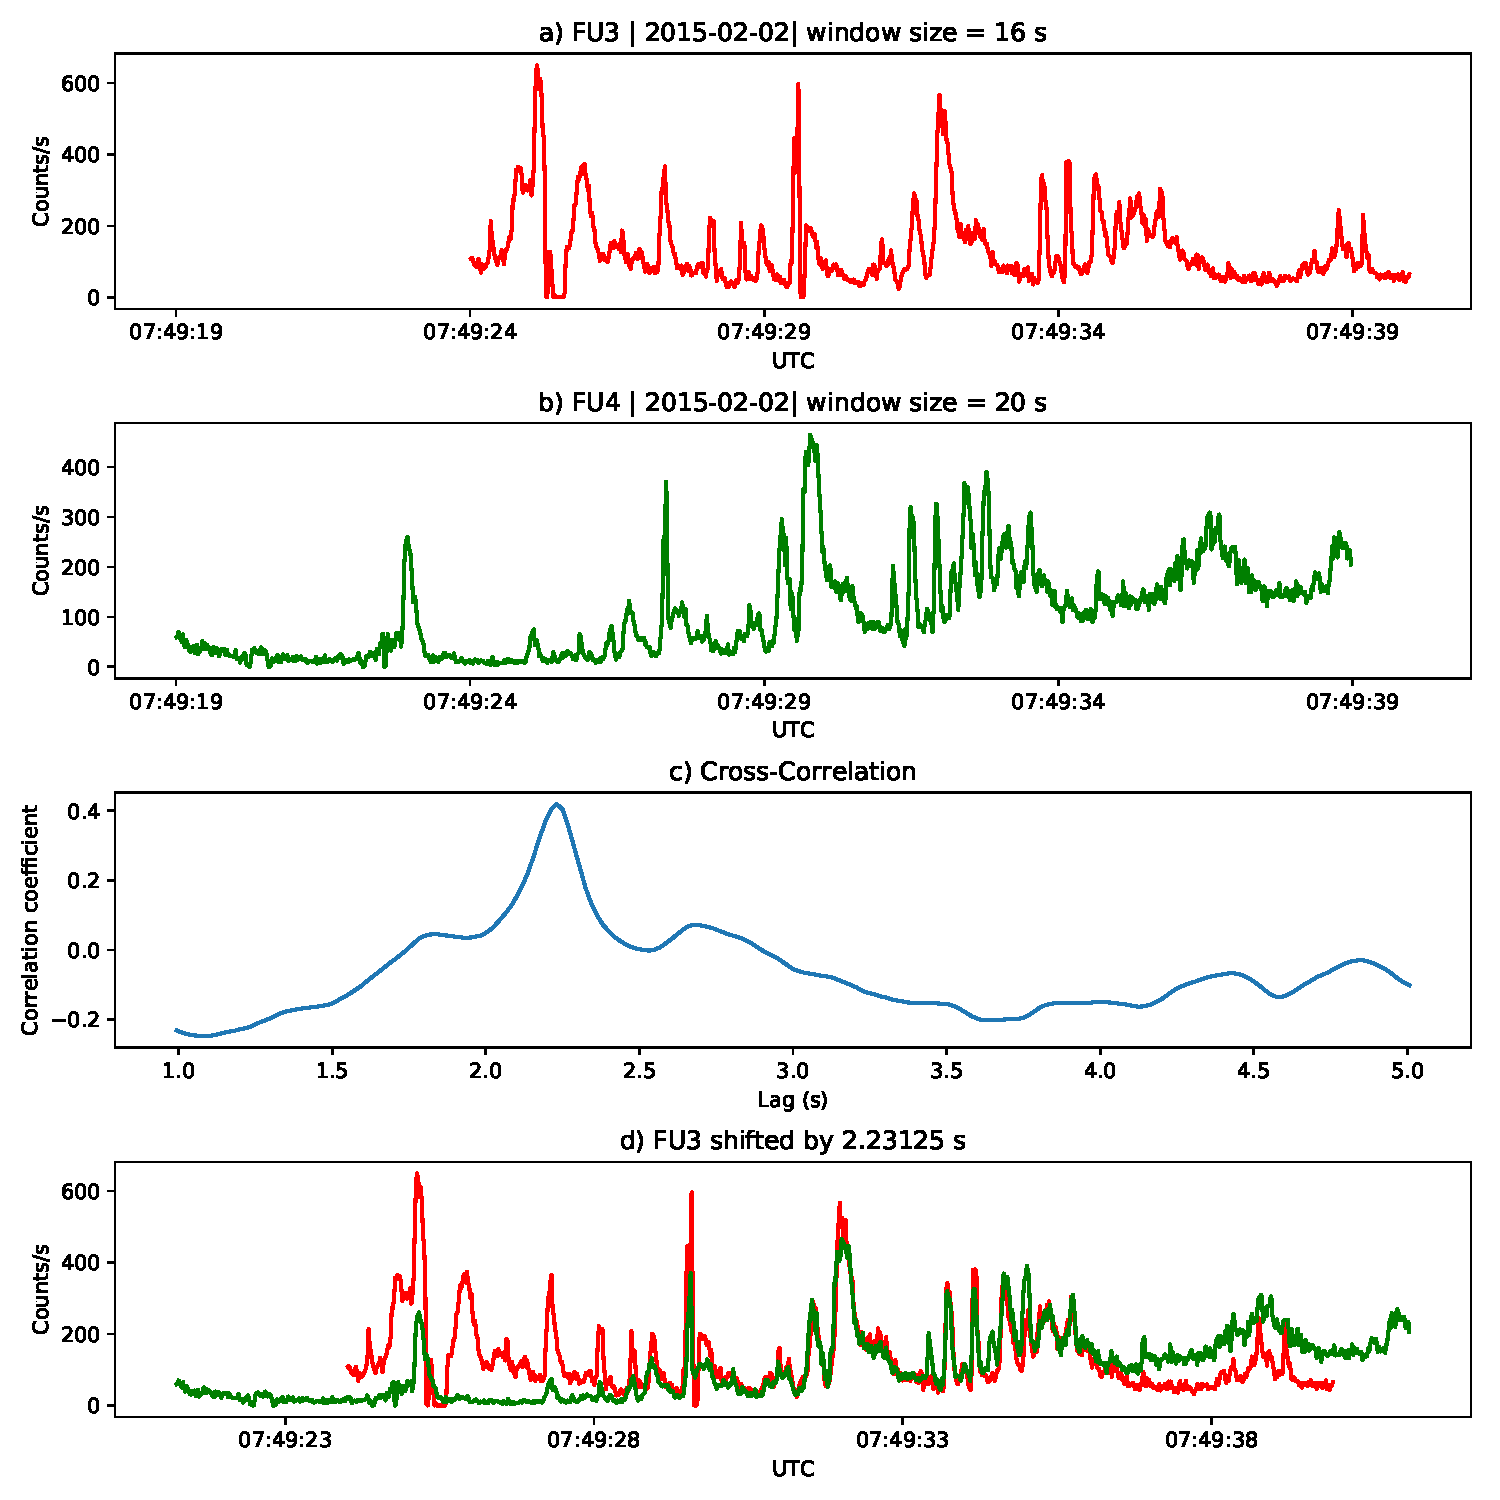
\includegraphics[width=0.8\textwidth]{2015-02-02_074931_microburst_crosscorr.pdf}
\caption{Cross-correlation time lag analysis applied to a train of microbursts. Panel (a) and (b) show the count rate from the lowest energy channel. Panel (c) shows the cross-correlation coefficient as a function of time lag. Panel (d) shows the shifted timeseries. Clock difference was 2.23 s.}
\label{figure_S1}
\end{figure}

\begin{figure}
\setfigurenum{S2} %%Change number for each figure
\noindent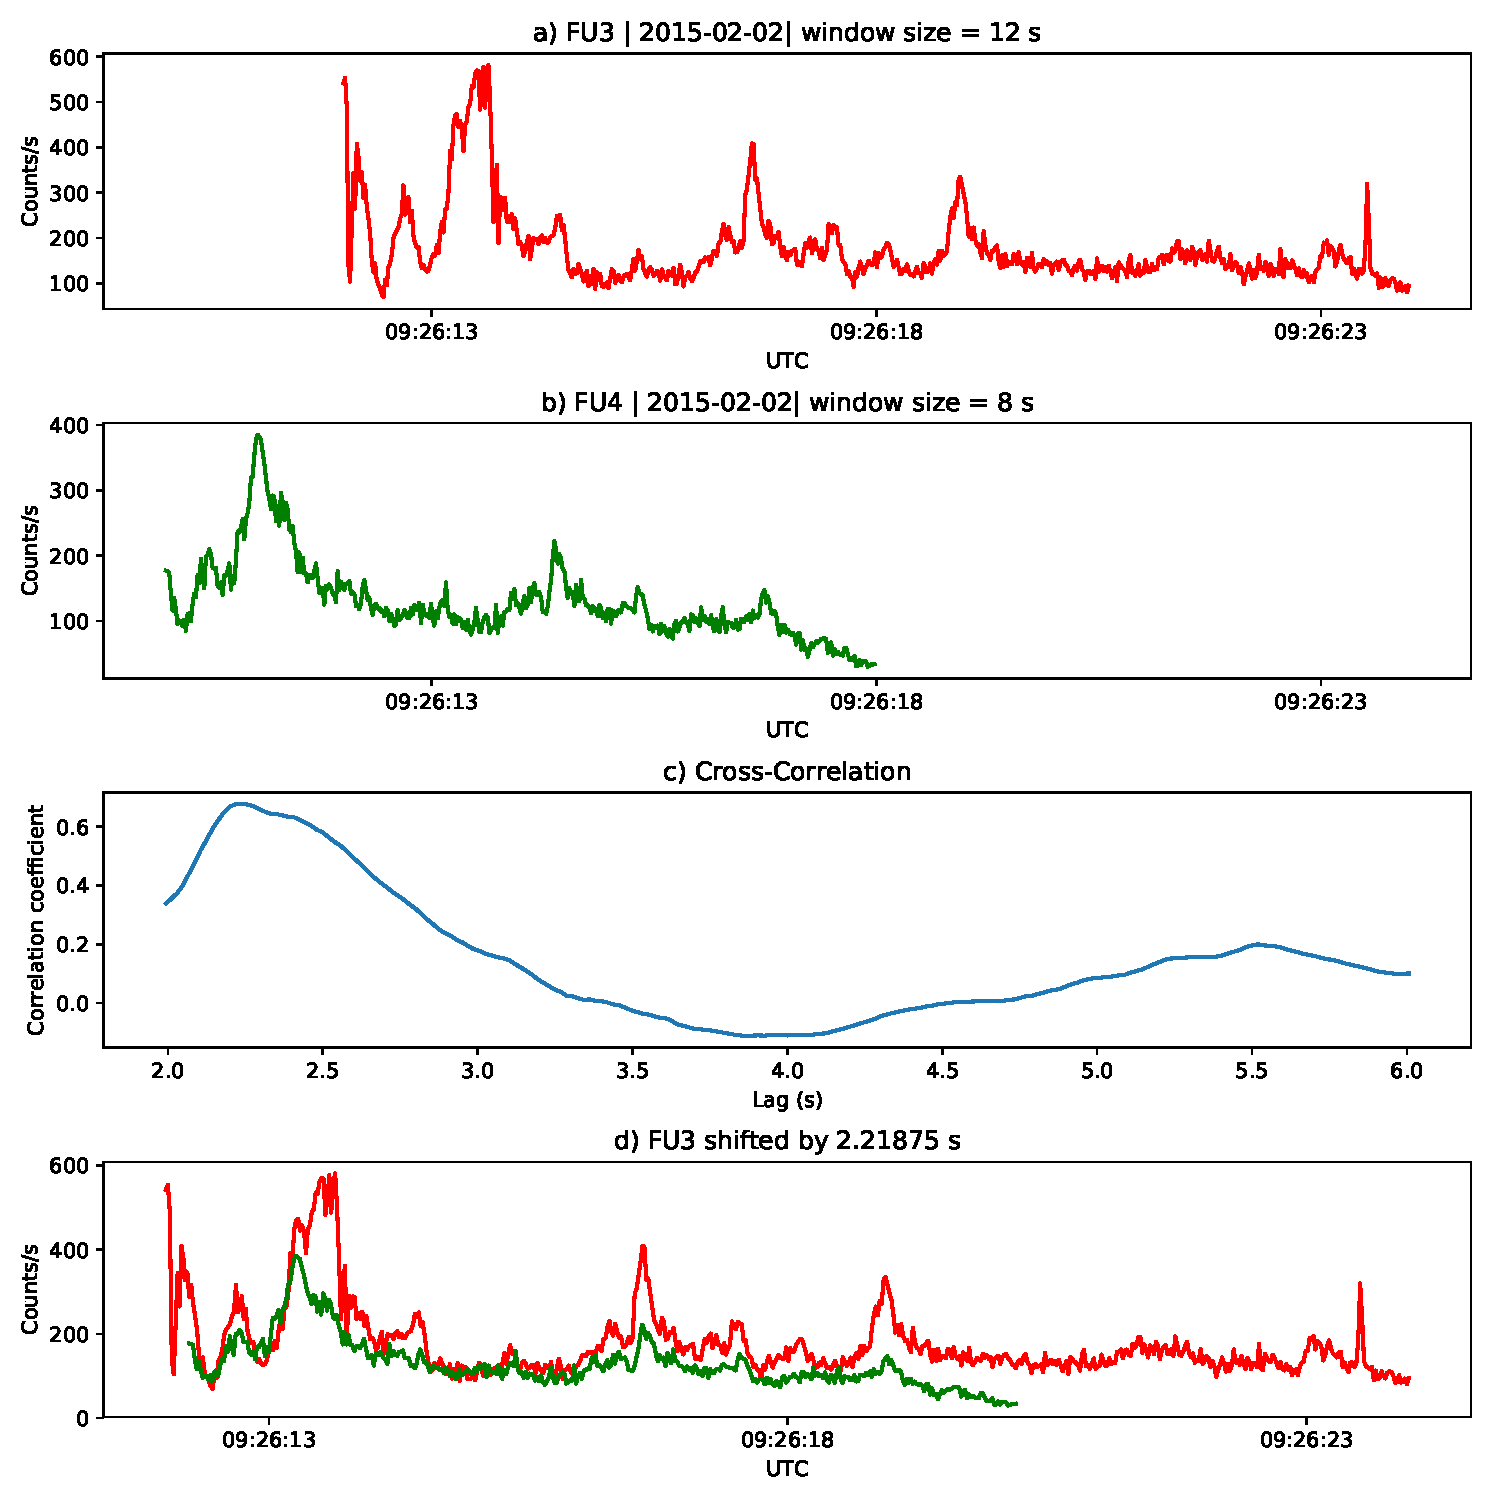
\includegraphics[width=0.8\textwidth]{2015-02-02_092613_microburst_crosscorr.pdf}
\caption{Same analysis as Fig. \ref{figure_S1} on a different time period. Clock difference was 2.21 s.}
\label{figure_S2}
\end{figure}

\begin{figure}
\setfigurenum{S3} %%Change number for each figure
\noindent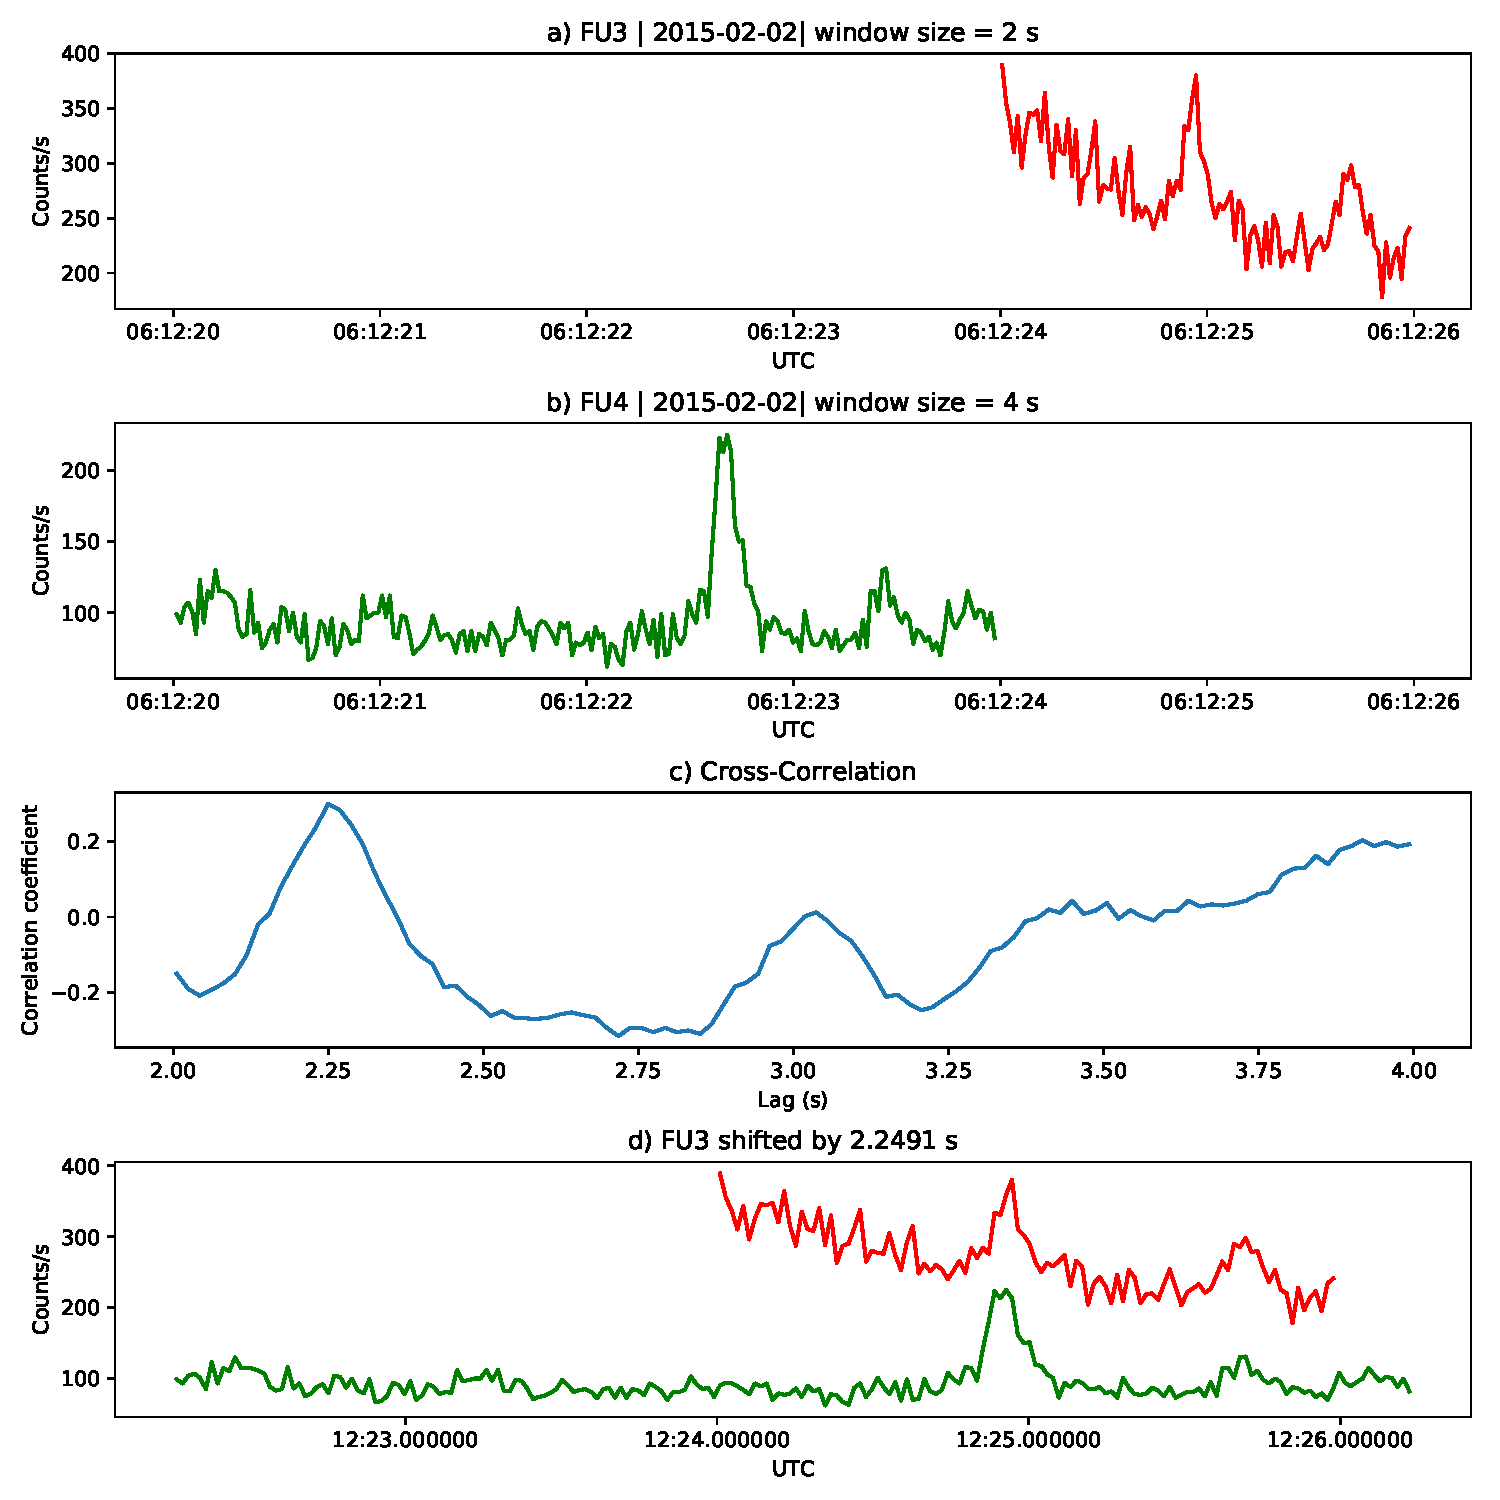
\includegraphics[width=0.8\textwidth]{2015-02-02_122300_microburst_crosscorr.pdf}
\caption{Same analysis as Fig. \ref{figure_S1} on a different time period. Clock difference was 2.25 s.}
\label{figure_S3}
\end{figure}

\begin{figure}
\setfigurenum{S4} %%Change number for each figure
\noindent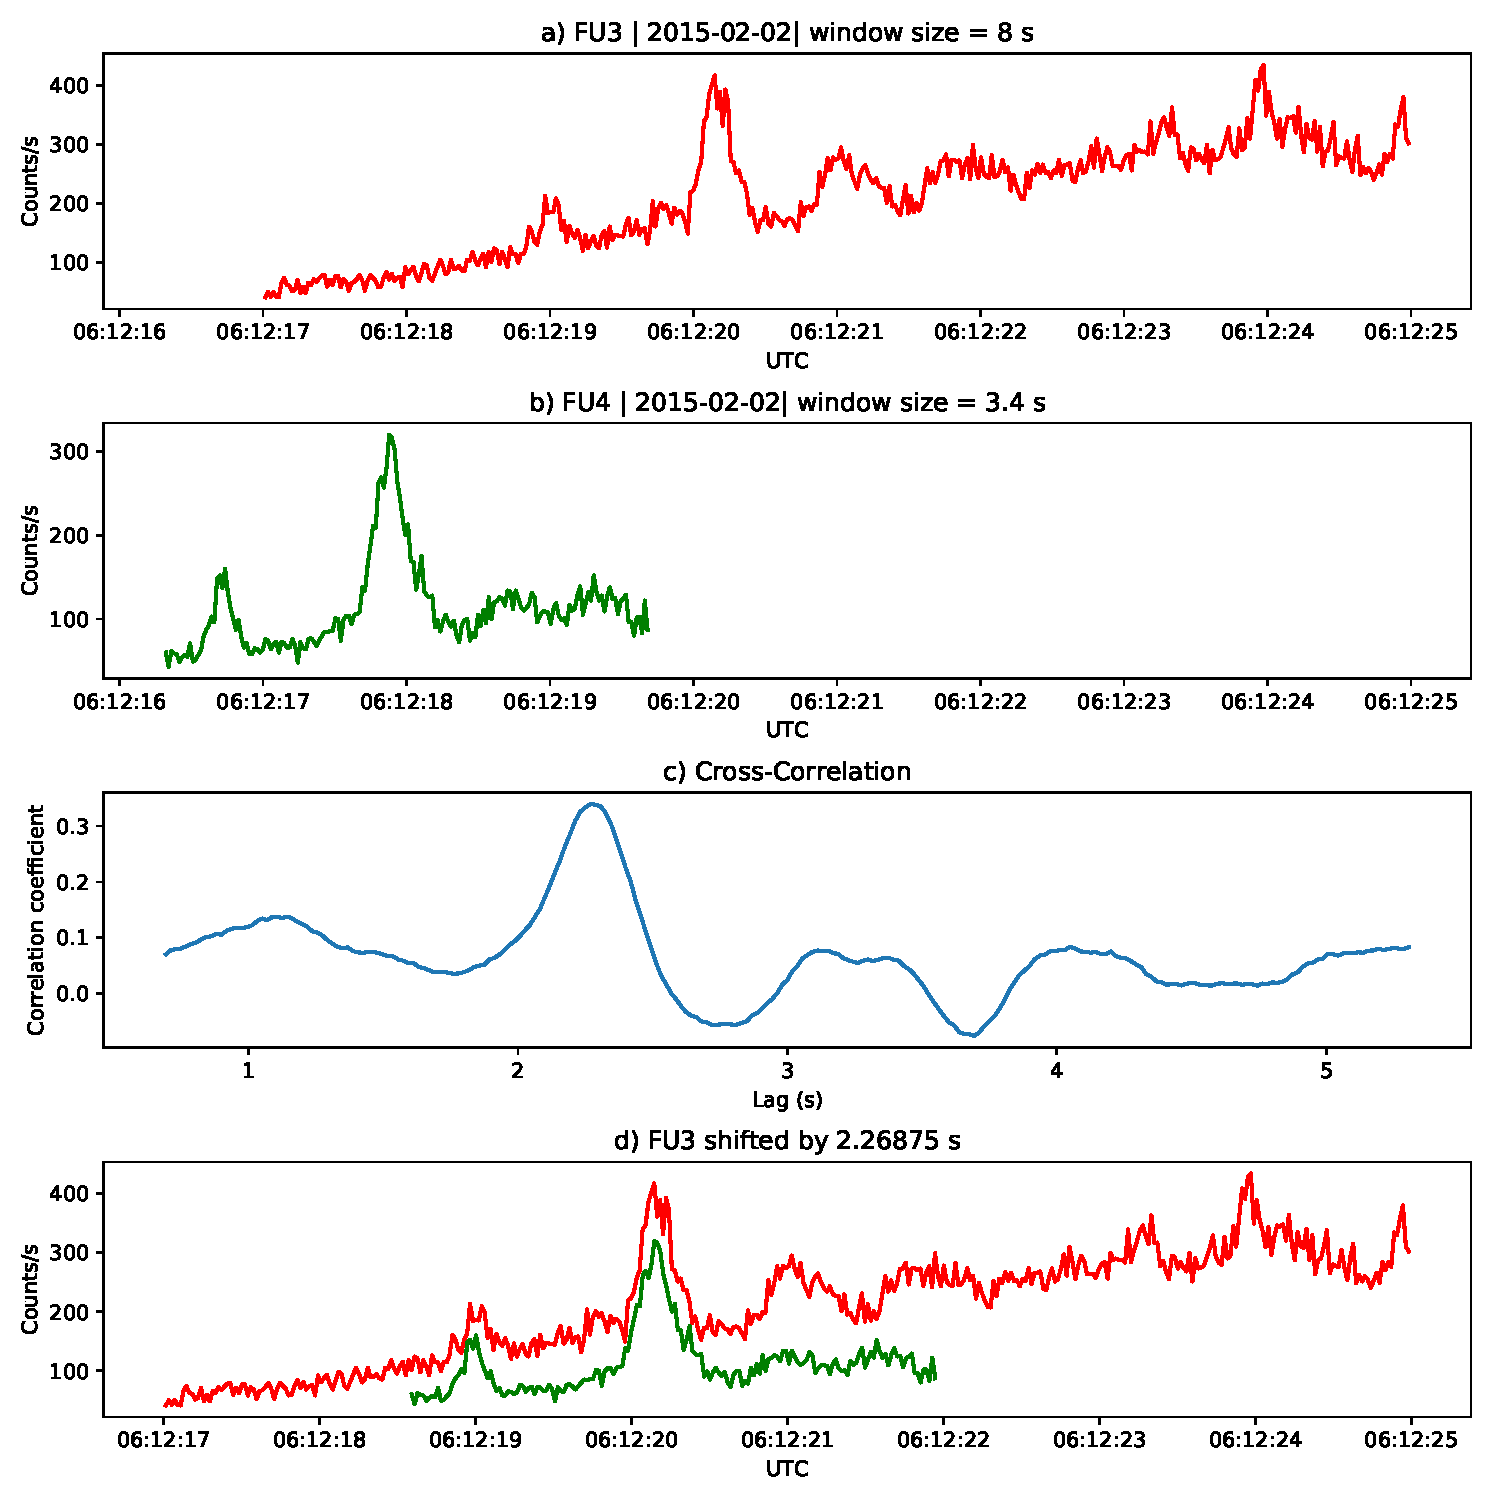
\includegraphics[width=0.8\textwidth]{2015-02-02_061217_microburst_crosscorr.pdf}
\caption{Same analysis as Fig. \ref{figure_S1} on a different time period. Clock difference was 2.27 s.}
\label{figure_S4}
\end{figure}

\begin{figure}
\setfigurenum{S5} %%Change number for each figure
\noindent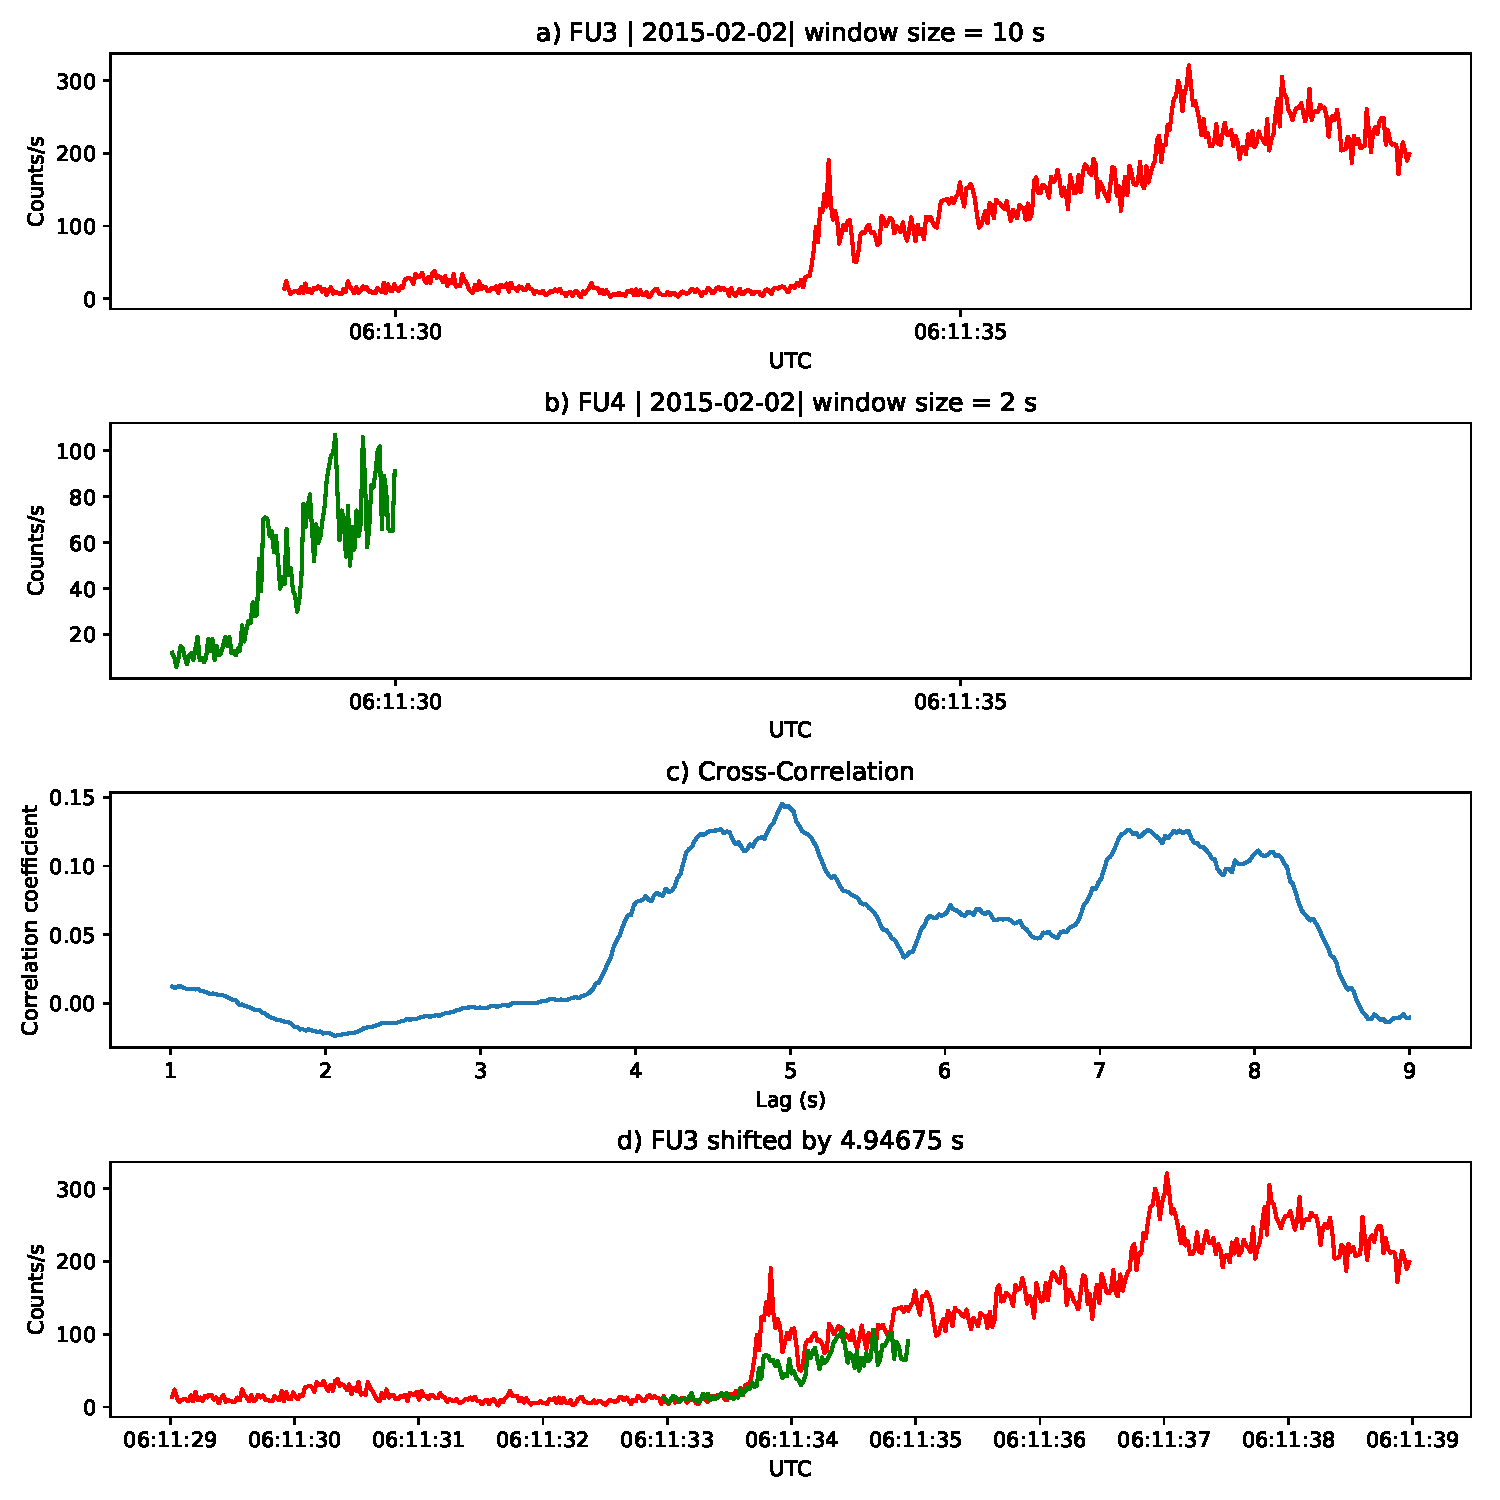
\includegraphics[width=0.8\textwidth]{2015-02-02_061129_stationary_crosscorr.pdf}
\caption{Same cross-correlation time lag analysis applied to stationary spatial structures. The cross-correlation lag between these events is a sum of the clock difference and time lag due to the spacecraft separation. The lag derived at this time was 4.95 s.}
\label{figure_S5}
\end{figure}

\begin{figure}
\setfigurenum{S6} %%Change number for each figure
\noindent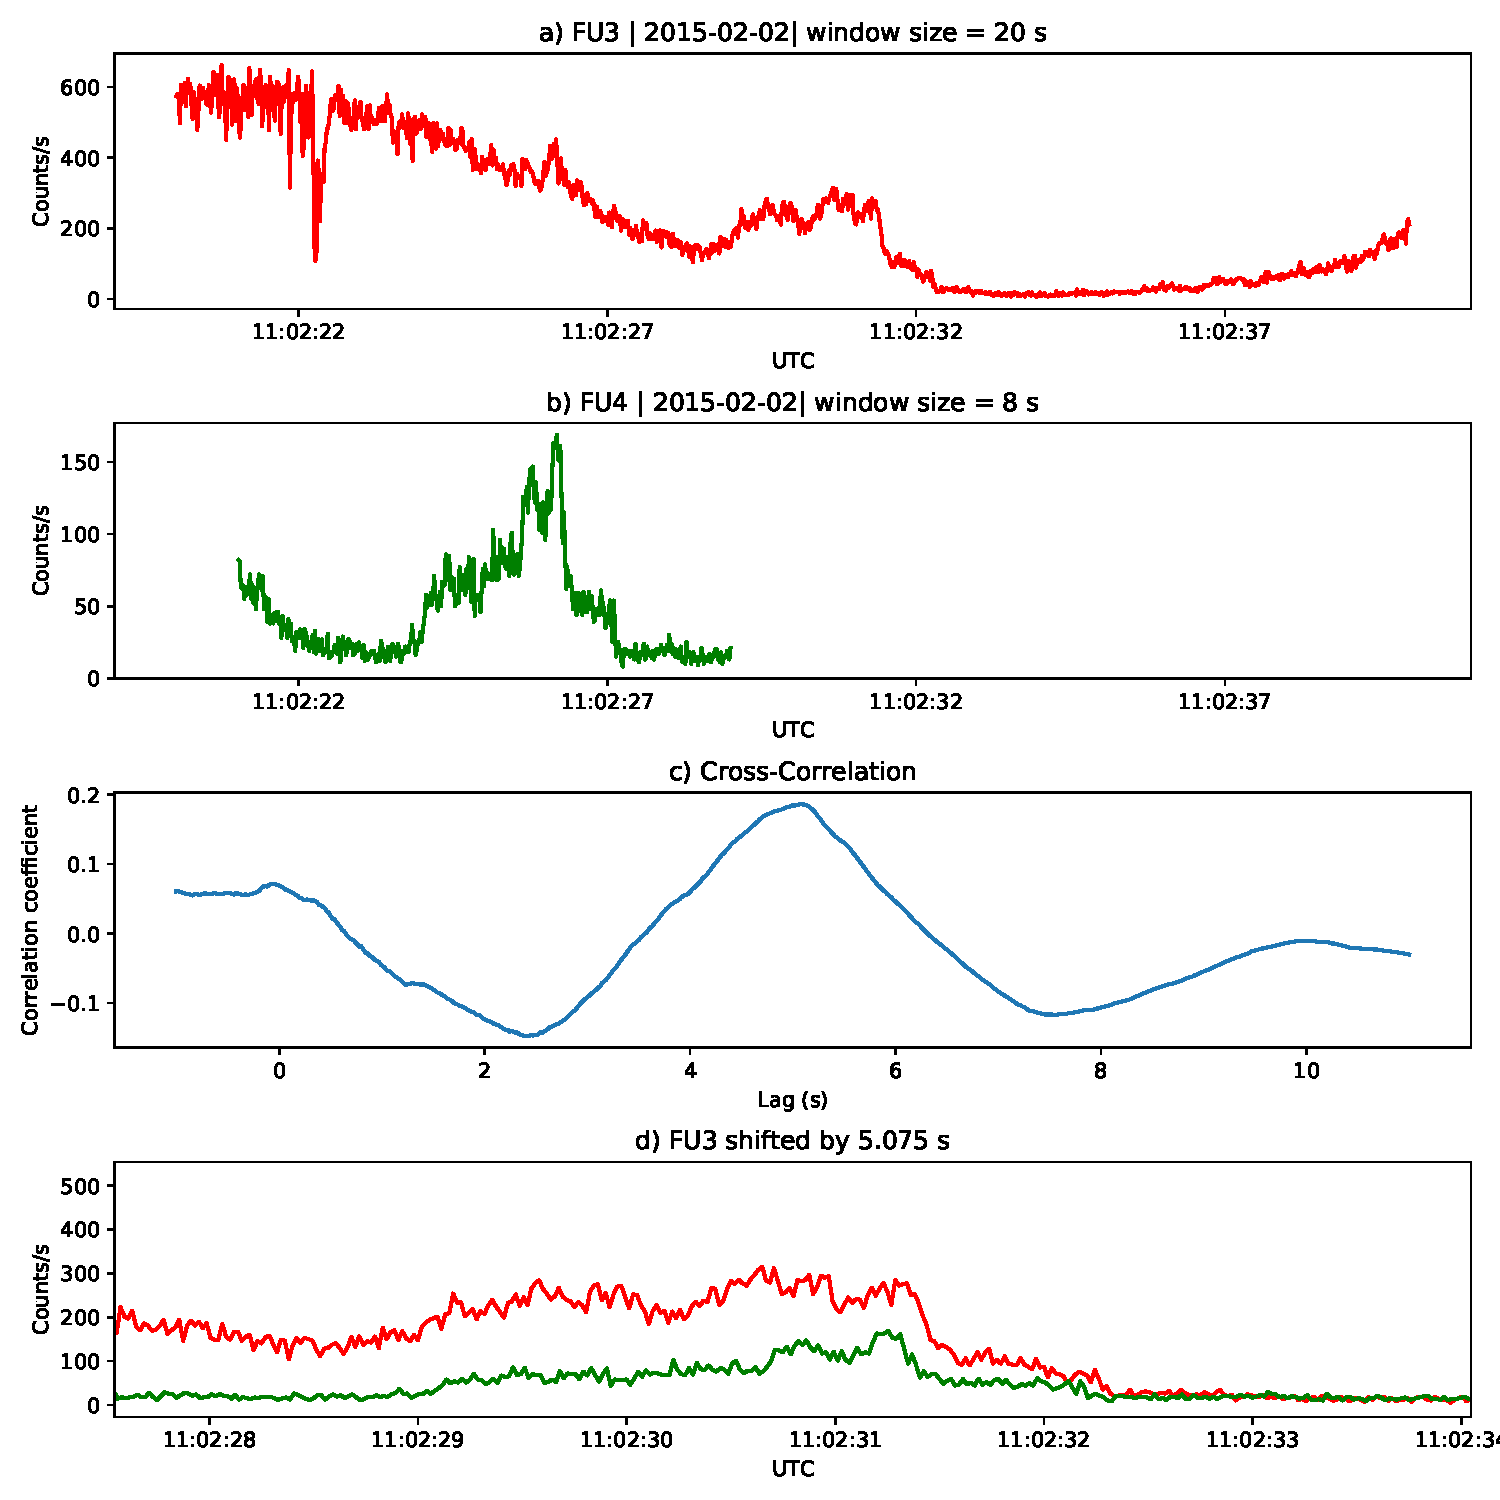
\includegraphics[width=0.8\textwidth]{2015-02-02_110228_stationary_crosscorr.pdf}
\caption{Same analysis as Fig. \ref{figure_S5} applied to a different stationary spatial feature. The lag derived at this time was 5.01 s.}
\label{figure_S6}
\end{figure}

\clearpage

%Type or paste text here. This should be additional explanatory text, such as: extended descriptions of results, full details of models, extended lists of acknowledgements etc.  It should not be additional discussion, analysis, interpretation or critique. It should not be an additional scientific experiment or paper.
%
%Repeat for any additional Supporting Text

%%Enter Data Set, Movie, and Audio captions here
%%EXAMPLE CAPTIONS

%Repeat for any additional Supporting audio files

%%% End of body of article:
%%%%%%%%%%%%%%%%%%%%%%%%%%%%%%%%%%%%%%%%%%%%%%%%%%%%%%%%%%%%%%%%
%
% Optional Notation section goes here
%
% Notation -- End each entry with a period.
% \begin{notation}
% Term & definition.\\
% Second term & second definition.\\
% \end{notation}
%%%%%%%%%%%%%%%%%%%%%%%%%%%%%%%%%%%%%%%%%%%%%%%%%%%%%%%%%%%%%%%%


%% ------------------------------------------------------------------------ %%
%%  REFERENCE LIST AND TEXT CITATIONS
%
% Either type in your references using
% \begin{thebibliography}{}
% \bibitem{}
% Text
% \end{thebibliography}
%
% Or,
%
% If you use BiBTeX for your references, please use the agufull08.bst file (available at % ftp://ftp.agu.org/journals/latex/journals/Manuscript-Preparation/) to produce your .bbl
% file and copy the contents into your paper here.
%
% Follow these steps:
% 1. Run LaTeX on your LaTeX file.
%
% 2. Make sure the bibliography style appears as \bibliographystyle{agufull08}. Run BiBTeX on your LaTeX
% file.
%
% 3. Open the new .bbl file containing the reference list and
%   copy all the contents into your LaTeX file here.
%
% 4. Comment out the old \bibliographystyle and \bibliography commands.
%
% 5. Run LaTeX on your new file before submitting.
%
% AGU does not want a .bib or a .bbl file. Please copy in the contents of your .bbl file here.

\begin{thebibliography}{}

\providecommand{\natexlab}[1]{#1}
\expandafter\ifx\csname urlstyle\endcsname\relax
  \providecommand{\doi}[1]{doi:\discretionary{}{}{}#1}\else
  \providecommand{\doi}{doi:\discretionary{}{}{}\begingroup
  \urlstyle{rm}\Url}\fi

\bibitem[{\textit{Hoots and Roehrich}(1980)}]{sgp4}
Hoots, F.~R., and R.~L. Roehrich (1980), Models for propagation of norad
  element sets, \textit{Tech. Rep.~3}, Spacetrack.
\end{thebibliography}

%Reference citation examples:

%...as shown by \textit{Kilby} [2008].
%...as shown by {\textit  {Lewin}} [1976], {\textit  {Carson}} [1986], {\textit  {Bartholdy and Billi}} [2002], and {\textit  {Rinaldi}} [2003].
%...has been shown [\textit{Kilby et al.}, 2008].
%...has been shown [{\textit  {Lewin}}, 1976; {\textit  {Carson}}, 1986; {\textit  {Bartholdy and Billi}}, 2002; {\textit  {Rinaldi}}, 2003].
%...has been shown [e.g., {\textit  {Lewin}}, 1976; {\textit  {Carson}}, 1986; {\textit  {Bartholdy and Billi}}, 2002; {\textit  {Rinaldi}}, 2003].

%...as shown by \citet{jskilby}.
%...as shown by \citet{lewin76}, \citet{carson86}, \citet{bartoldy02}, and \citet{rinaldi03}.
%...has been shown \citep{jskilbye}.
%...has been shown \citep{lewin76,carson86,bartoldy02,rinaldi03}.
%...has been shown \citep [e.g.,][]{lewin76,carson86,bartoldy02,rinaldi03}.
%
% Please use ONLY \citet and \citep for reference citations.
% DO NOT use other cite commands (e.g., \cite, \citeyear, \nocite, \citealp, etc.).

%% ------------------------------------------------------------------------ %%
%
%  END ARTICLE
%
%% ------------------------------------------------------------------------ %%
\end{article}
\clearpage

% Delete all unused file types below. Copy/paste for multiples of each file type as needed.

% enter figures and tables here:
%
% EXAMPLE FIGURE
% ---------------
% \begin{figure}
%\setfigurenum{S1} %%Change number for each figure
% \noindent\includegraphics[width=20pc]{samplefigure.eps}
%\caption{Caption text here}
 %\label{figure_label}
 %\end{figure}

% ---------------
% EXAMPLE TABLE
%
%\begin{table}
%\settablenum{S1} %%Change number for each table
%\caption{Time of the Transition Between Phase 1 and Phase 2\tablenotemark{a}}
%\centering
%\begin{tabular}{l c}
%\hline
% Run  & Time (min)  \\
%\hline
%  $l1$  & 260   \\
%  $l2$  & 300   \\
%  $l3$  & 340   \\
%  $h1$  & 270   \\
%  $h2$  & 250   \\
%  $h3$  & 380   \\
%  $r1$  & 370   \\
%  $r2$  & 390   \\
%\hline
%\end{tabular}
%\tablenotetext{a}{Footnote text here.}
%\end{table}
% ---------------
%
% EXAMPLE LARGE TABLE (UPLOADED SEPARATELY)
%\begin{table}
%\settablenum{S1} %%Change number for each table
%\caption{Time of the Transition Between Phase 1 and Phase 2\tablenotemark{a}}
%\end{table}


\end{document}

%%%%%%%%%%%%%%%%%%%%%%%%%%%%%%%%%%%%%%%%%%%%%%%%%%%%%%%%%%%%%%%

More Information and Advice:

%% ------------------------------------------------------------------------ %%
%
%  SECTION HEADS
%
%% ------------------------------------------------------------------------ %%

% Capitalize the first letter of each word (except for
% prepositions, conjunctions, and articles that are
% three or fewer letters).

% AGU follows standard outline style; therefore, there cannot be a section 1 without
% a section 2, or a section 2.3.1 without a section 2.3.2.
% Please make sure your section numbers are balanced.
% ---------------
% Level 1 head
%
% Use the \section{} command to identify level 1 heads;
% type the appropriate head wording between the curly
% brackets, as shown below.
%
%An example:
%\section{Level 1 Head: Introduction}
%
% ---------------
% Level 2 head
%
% Use the \subsection{} command to identify level 2 heads.
%An example:
%\subsection{Level 2 Head}
%
% ---------------
% Level 3 head
%
% Use the \subsubsection{} command to identify level 3 heads
%An example:
%\subsubsection{Level 3 Head}
%
%---------------
% Level 4 head
%
% Use the \subsubsubsection{} command to identify level 3 heads
% An example:
%\subsubsubsection{Level 4 Head} An example.
%
%% ------------------------------------------------------------------------ %%
%
%  IN-TEXT LISTS
%
%% ------------------------------------------------------------------------ %%
%
% Do not use bulleted lists; enumerated lists are okay.
% \begin{enumerate}
% \item
% \item
% \item
% \end{enumerate}
%
%% ------------------------------------------------------------------------ %%
%
%  EQUATIONS
%
%% ------------------------------------------------------------------------ %%

% Single-line equations are centered.
% Equation arrays will appear left-aligned.

Math coded inside display math mode \[ ...\]
 will not be numbered, e.g.,:
 \[ x^2=y^2 + z^2\]

 Math coded inside \begin{equation} and \end{equation} will
 be automatically numbered, e.g.,:
 \begin{equation}
 x^2=y^2 + z^2
 \end{equation}

% IF YOU HAVE MULTI-LINE EQUATIONS, PLEASE
% BREAK THE EQUATIONS INTO TWO OR MORE LINES
% OF SINGLE COLUMN WIDTH (20 pc, 8.3 cm)
% using double backslashes (\\).

% To create multiline equations, use the
% \begin{eqnarray} and \end{eqnarray} environment
% as demonstrated below.
\begin{eqnarray}
  x_{1} & = & (x - x_{0}) \cos \Theta \nonumber \\
        && + (y - y_{0}) \sin \Theta  \nonumber \\
  y_{1} & = & -(x - x_{0}) \sin \Theta \nonumber \\
        && + (y - y_{0}) \cos \Theta.
\end{eqnarray}

%If you don't want an equation number, use the star form:
%\begin{eqnarray*}...\end{eqnarray*}

% Break each line at a sign of operation
% (+, -, etc.) if possible, with the sign of operation
% on the new line.

% Indent second and subsequent lines to align with
% the first character following the equal sign on the
% first line.

% Use an \hspace{} command to insert horizontal space
% into your equation if necessary. Place an appropriate
% unit of measure between the curly braces, e.g.
% \hspace{1in}; you may have to experiment to achieve
% the correct amount of space.


%% ------------------------------------------------------------------------ %%
%
%  EQUATION NUMBERING: COUNTER
%
%% ------------------------------------------------------------------------ %%

% You may change equation numbering by resetting
% the equation counter or by explicitly numbering
% an equation.

% To explicitly number an equation, type \eqnum{}
% (with the desired number between the brackets)
% after the \begin{equation} or \begin{eqnarray}
% command.  The \eqnum{} command will affect only
% the equation it appears with; LaTeX will number
% any equations appearing later in the manuscript
% according to the equation counter.
%

% If you have a multiline equation that needs only
% one equation number, use a \nonumber command in
% front of the double backslashes (\\) as shown in
% the multiline equation above.

%% ------------------------------------------------------------------------ %%
%
%  SIDEWAYS FIGURE AND TABLE EXAMPLES
%
%% ------------------------------------------------------------------------ %%
%
% For tables and figures, add \usepackage{rotating} to the paper and add the rotating.sty file to the folder.
% AGU prefers the use of {sidewaystable} over {landscapetable} as it causes fewer problems.
%
% \begin{sidewaysfigure}
% \includegraphics[width=20pc]{samplefigure.eps}
% \caption{caption here}
% \label{label_here}
% \end{sidewaysfigure}
%
%
%
% \begin{sidewaystable}
% \caption{}
% \begin{tabular}
% Table layout here.
% \end{tabular}
% \end{sidewaystable}
%
%
